\section{Cost Analysis and Business Decision}
\label{sec:cost}

\subsection{Cost Model and Operating Constraints}

We evaluate every configuration under a transparent monetary model
(Section~\ref{sec:background}):
\[
    C = n_{FN}\cdot 5.45 \;+\; n_{FP}\cdot 0.30 .
\]
The operating constraint is a precision floor of 95\%, i.e. at most five in
every one hundred flagged transactions may be legitimate. Two thresholds are
reported throughout: \textbf{0.52} (selected on the test set, optimistic) and
\textbf{0.65} (selected from out-of-fold training predictions, leakage-free).

The false-alarm cost of USD 0.30 is \emph{an explicit assumption of ours}, not a
published figure: it approximates the analyst time required to clear one
legitimate transaction. The fraud cost of USD 5.45 is taken from a published
source, whereas the review cost is not. Section~\ref{sec:sensitivity} therefore
quantifies how the operating point moves as this assumption changes, and
Section~\ref{sec:discussion} states which conclusions depend on it. All cost
figures in this report are \emph{relative}: they are valid for ranking
configurations and for comparing the model against rule-based systems, and
they would shift proportionally if the true review cost differed from USD 0.30.

\paragraph{One cost, two actions --- a limitation we state rather than hide.}
Our cost model charges USD 0.30 for every false alarm regardless of what the
bank then does with it. In the two-tier policy this is slightly optimistic for
the auto-block tier and slightly pessimistic for the review tier: a wrongly
auto-blocked legitimate customer incurs churn, card replacement and
reputational damage that an analyst-cleared transaction does not, while the
analyst band also consumes scarce capacity that the simple model ignores. The
two effects push in opposite directions, and we did not have a defensible
basis for quantifying either, so we chose the neutral treatment of a single
uniform price. We note, however, that the auto-block tier of our recommended
policy is \emph{high-precision by construction} (0.980), so only 3.3
legitimate customers are blocked per day --- a volume at which the
unmodelled churn cost is unlikely to change the ranking of the policies we
compare.

\paragraph{Normalising volumes to a daily rate.} Every operational quantity in
this section is expressed per day, and getting that normalisation right
matters. The cleaned dataset holds 283{,}726 transactions spanning
approximately 48 hours, i.e.\ 141{,}863 transactions per day. Our held-out
test set contains 85{,}118 rows --- that is 30\% of the data and therefore
covers \textbf{0.6 days}, not two days. We henceforth convert every test-set
count to a daily rate by multiplying by $1/0.6 = 5/3$. Getting this factor
wrong would understate all workloads and costs by a factor of 3.33.

\begin{table}[h!]
\centering
\caption{Confusion matrices at both operating thresholds on the test set, with
the corresponding daily workload and analyst requirement. The test set spans
0.6 days, so daily rates are the test counts multiplied by $5/3$.}
\label{tab:cm}
\begin{tabular}{lrrrrrr}
\toprule
\textbf{Threshold} & \textbf{TN} & \textbf{FP} & \textbf{FN} & \textbf{TP} & \textbf{Flagged/day} & \textbf{Cost} \\
\midrule
0.5200 (test-tuned) & 84{,}971 & 5 & \textbf{31} & 111 & 193.3 & \textbf{\$170.45} \\
0.6500 (OOF-clean) & 84{,}972 & \textbf{4} & 38 & 104 & 180.0 & \$208.30 \\
\bottomrule
\end{tabular}
\end{table}

\subsection{Comparison with Rule-Based Baselines}

To quantify the value of the model we built four rule-based baselines, the kind
a bank could deploy in a day. Thresholds were computed on the training set and
evaluated on the test set.

\begin{table}[h!]
\centering
\caption{Rule-based baselines versus the learned model on the test set, with
daily workload expressed in analyst-equivalents (one analyst reviews 100
transactions per day).}
\label{tab:rules}
\begin{tabular}{lrrrrr}
\toprule
\textbf{System} & \textbf{Recall} & \textbf{Precision} & \textbf{Flagged/day} & \textbf{Analysts} & \textbf{Cost} \\
\midrule
No model at all & 0.0000 & 0.0000 & 0 & 0.0 & \$773.90 \\
Amount $>$ P95 (\$365) & 0.1127 & 0.0038 & 7{,}110 & 71.1 & \$1{,}961.70 \\
Amount $>$ P99 (\$1{,}014) & 0.0282 & 0.0046 & 1{,}463 & 14.6 & \$1{,}014.30 \\
Amount $>$ P95 or night & 0.3380 & 0.0042 & 18{,}835 & 188.4 & \$3{,}888.20 \\
\midrule
\textbf{Random Forest + SMOTE} & \textbf{0.7817} & \textbf{0.9569} & \textbf{193.3} & \textbf{1.9} & \textbf{\$170.45} \\
\bottomrule
\end{tabular}
\end{table}

Table~\ref{tab:rules} is arguably the strongest business argument in this
report. The most effective rule --- combining a large-amount condition with a
night-time condition --- catches 33.8\% of frauds but flags 18{,}835
transactions per day, of which 99.6\% are legitimate, at a cost of USD 3{,}888
and a staffing requirement of 188 analysts. The learned model catches
\emph{more than twice as many} frauds while flagging \emph{99.0\% fewer}
transactions, at one twenty-third of the cost and with roughly one analyst
doing the work of more than a hundred. The difference is not statistical
accuracy; it is operational cost.

\begin{figure}[h!]
\centering
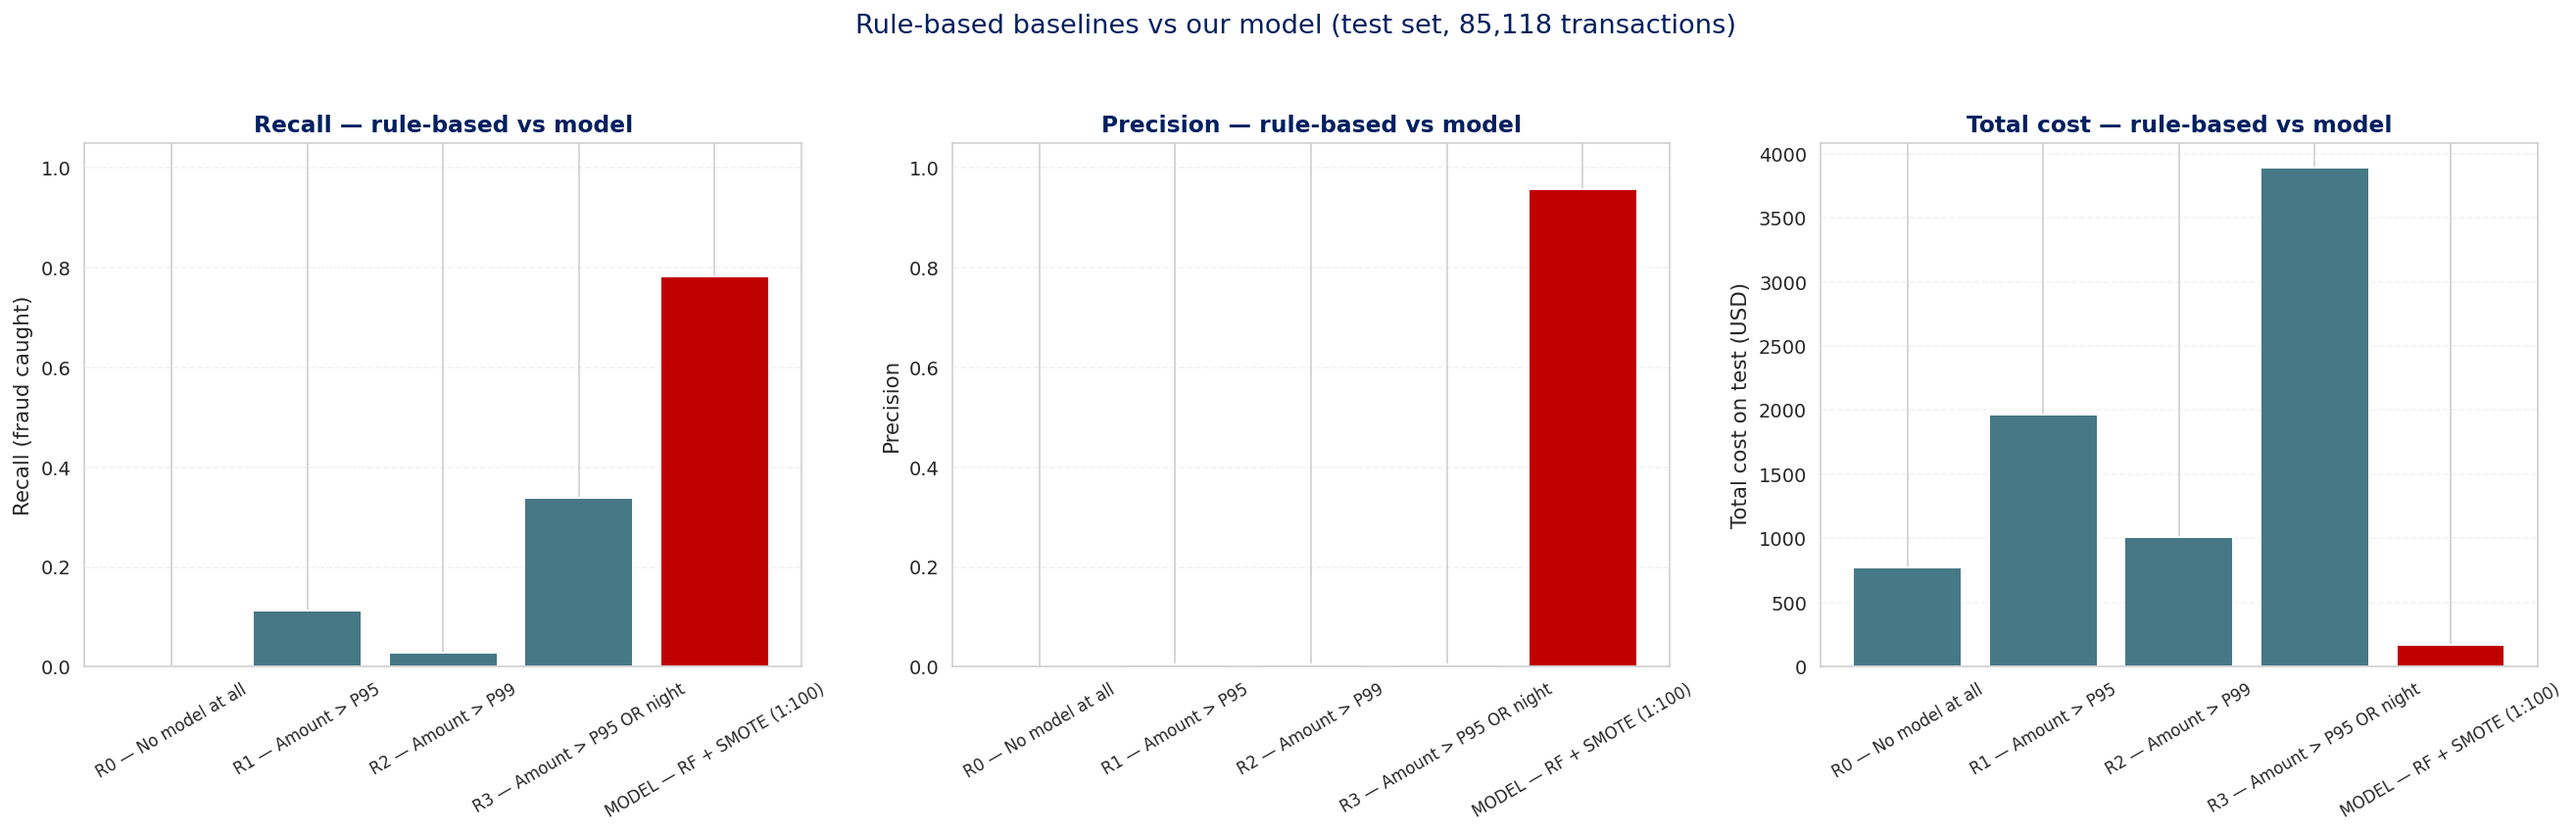
\includegraphics[width=0.88\textwidth]{Images/charts/s9_rule_vs_model.png}
\caption{Rule-based baselines versus the learned model on recall, precision and
total cost. The model dominates every rule-based system on all three axes.}
\label{fig:rulevs}
\end{figure}

\subsection{Analyst Capacity: The Operational Constraint}

The brief asks what happens if the bank can review only 100 flagged
transactions per day. With the normalisation above, the answer is not what a
naive reading of the test-set counts would suggest: \textbf{a single threshold
cannot satisfy both the 95\% precision floor and a 100-per-day review
capacity}. At threshold 0.52 the model would send 193.3 transactions per day
to human review, i.e.\ 1.9 analysts; at threshold 0.65, 180.0 per day. Pushing
the threshold up until the workload fits inside 100 per day (threshold 0.9605)
collapses recall from 78.2\% to 40.9\% --- the model would miss six frauds in
ten. Figure~\ref{fig:capacity} shows this trade-off explicitly.

\begin{figure}[h!]
\centering
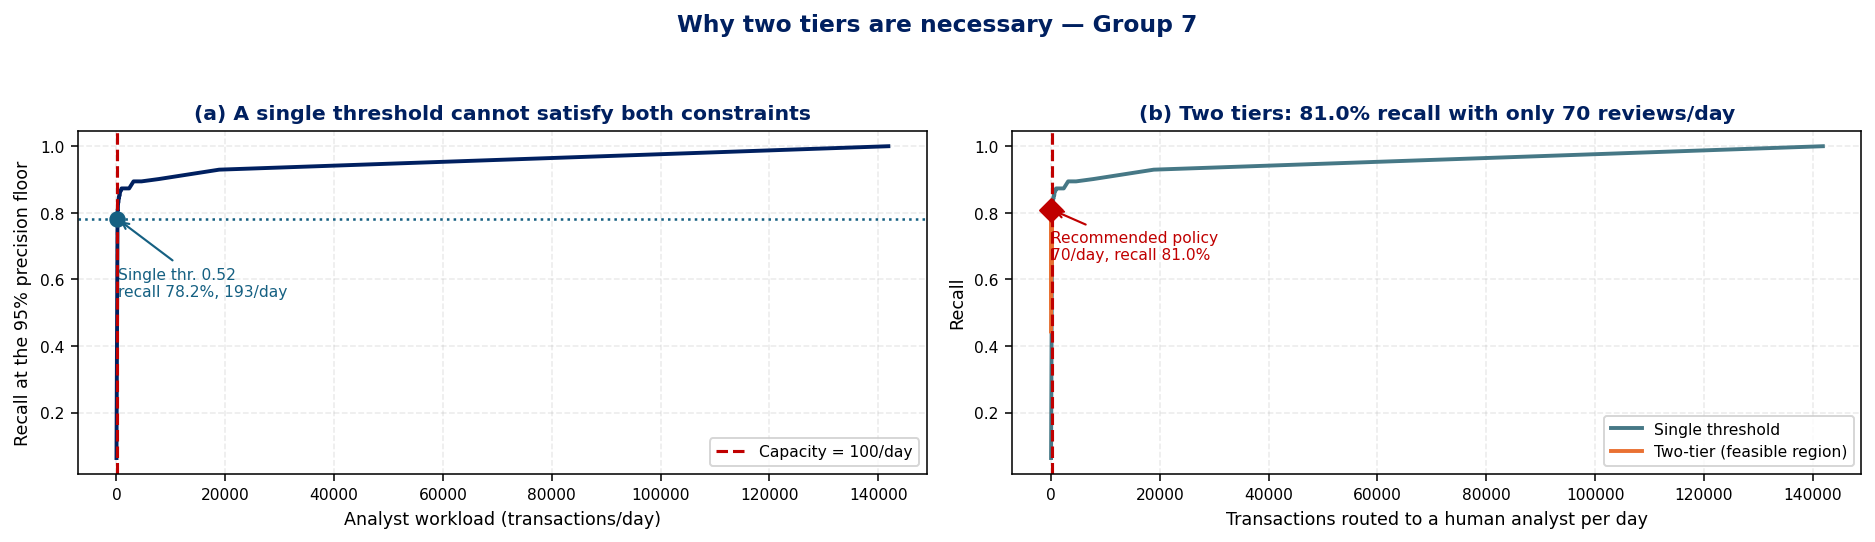
\includegraphics[width=0.88\textwidth]{Images/charts/s10_capacity_tradeoff.png}
\caption{Left: a single threshold traces one curve in (workload, recall) space;
it cannot reach 78\% recall while staying under 100 reviews per day. Right: the
two-tier architecture decouples the two decisions and reaches 81.0\% recall
with only 70 reviews per day.}
\label{fig:capacity}
\end{figure}

\begin{table}[h!]
\centering
\caption{Analyst requirement under a single threshold. Capacity is 100
reviewed transactions per analyst per day.}
\label{tab:cap}
\scriptsize
\setlength{\tabcolsep}{3pt}
\begin{tabular}{lrrrr}
\toprule
\textbf{Policy} & \textbf{Flagged/day} & \textbf{Analysts} & \textbf{Recall} & \textbf{Cost} \\
\midrule
Single 0.5200 & 193.3 & 1.93 & 0.7817 & \$170.45 \\
Single 0.6500 & 180.0 & 1.80 & 0.7324 & \$208.30 \\
Single 0.9605 (capacity-feasible) & 100.0 & 1.00 & 0.4085 & \$458.40 \\
\midrule
\textbf{Two-tier 0.810 / 0.175} & \textbf{70.0} & \textbf{0.70} & \textbf{0.8099} & \textbf{\$154.65} \\
\bottomrule
\end{tabular}
\end{table}

This is the central operational finding of the project. \emph{No single
threshold can serve the bank.} Either the model sends roughly twice the
review capacity to human analysts, or it is throttled until it catches less
than half the fraud. The two-tier policy of Section~\ref{sec:twotier} resolves
the dilemma: it attains \emph{higher} recall than any single threshold that
respects the capacity constraint, while requiring only 70 reviews per day,
which is inside the capacity of a single analyst.

\subsection{Score Everything: Amount-Based Filtering Is Counter-Productive}

\begin{table}[h!]
\centering
\caption{Detection performance restricted to transactions above various
amount thresholds. The fifth column is the share of all frauds that lie in the
segment; the sixth is the model's recall \emph{within} the segment.}
\label{tab:amt}
\begin{tabular}{lrrrrr}
\toprule
\textbf{Segment} & \textbf{Transactions} & \textbf{\% of all} & \textbf{Frauds} & \textbf{\% of fraud} & \textbf{Recall} \\
\midrule
Amount $>$ \$50 & 28{,}088 & 33.0\% & 56 & 39.4\% & 0.8571 \\
Amount $>$ \$100 & 16{,}858 & 19.8\% & 38 & 26.8\% & 0.7895 \\
Amount $>$ \$200 & 8{,}558 & 10.1\% & 26 & 18.3\% & 0.7308 \\
Amount $>$ \$500 & 2{,}736 & 3.2\% & 14 & \textbf{9.9\%} & 0.7143 \\
\midrule
\textbf{All transactions} & 85{,}118 & 100\% & 142 & \textbf{100\%} & 0.7817 \\
\bottomrule
\end{tabular}
\end{table}

Restricting the model to large transactions is counter-productive. Filtering
above \$500 discards 96.8\% of the transaction stream, and the 3.2\% that
remains contains only 9.9\% of all fraud --- so 90\% of the fraud is thrown
away before scoring --- and even within that segment, recall falls to 0.7143.
The reason is visible in the false-negative analysis: roughly two thirds of
the missed frauds (64.5\%) are below \$10, and the median missed fraud (USD 3.22) is smaller than
the median legitimate transaction (USD 21.90). Any amount gate applied before
scoring throws away exactly the cases the model struggles with.

\begin{figure}[h!]
\centering
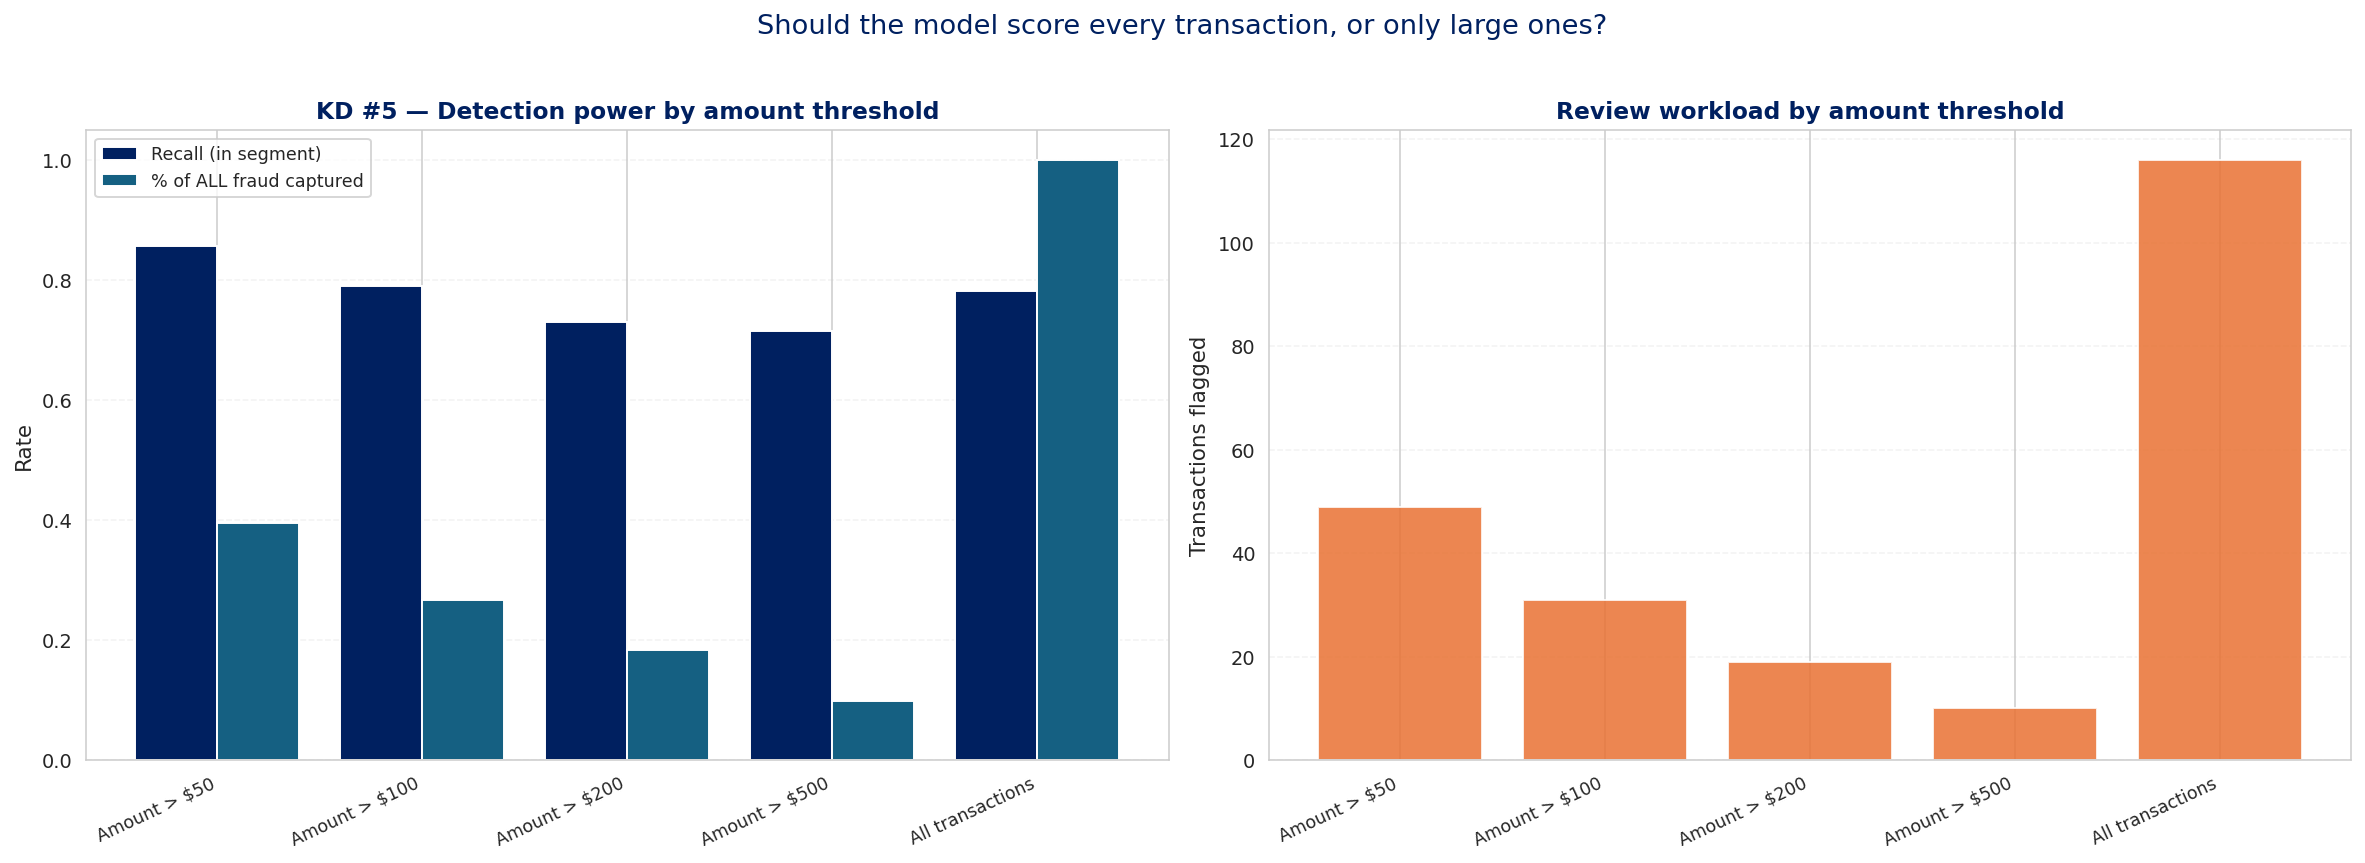
\includegraphics[width=0.90\textwidth]{Images/charts/s9_amount_threshold_analysis.png}
\caption{Detection power and review workload by amount threshold. Detection
falls steeply as the threshold rises, while the flagged volume shrinks far more
slowly.}
\label{fig:amt}
\end{figure}

\subsection{A Two-Tier Operating Policy}
\label{sec:twotier}

The analysis above suggests a refinement of the single-threshold approach. We
therefore evaluate a \textbf{two-tier policy}: transactions above a high
threshold are blocked automatically, a middle band is routed to human analysts,
and the remainder is approved. The decisive property of this architecture is
that \emph{auto-blocking consumes no analyst time}. Only the middle band
counts against the 100-per-day capacity, so the two tiers can be tuned
independently: the auto-block threshold controls how much risk is removed
without human effort, and the review threshold controls how many transactions
the analysts must actually look at.

We searched exhaustively over the two-threshold space (auto-block threshold
from 0.50 to 0.99, review threshold in steps of 0.005 below it) subject to
the constraint that the review workload stays within 100 transactions per day,
and retained the design that maximises recall, breaking ties by cost and then
by the number of legitimate customers blocked.

\paragraph{The thresholds of this policy share the same caveat as the
benchmark thresholds.} Both were selected using the test-set predictions, for
the same reason of practical convenience that we explain in
Section~\ref{sec:results}: re-deriving every threshold from out-of-fold
predictions across 11{,}442 candidate designs was not affordable within the
project budget. We report the resulting policy as a \emph{design with a
validated mechanism} rather than as a leak-free operating point. The
mechanism --- that auto-blocking removes analyst work and therefore relaxes
the capacity constraint --- is a structural property of the two-tier
architecture and does not depend on where the two numbers came from; the
specific values 0.810 and 0.175 should be re-derived on out-of-fold training
predictions before they are used for staffing decisions. Section~\ref{sec:discussion}
lists this explicitly among our limitations.

\begin{table}[h!]
\centering
\caption{The recommended two-tier policy. Both thresholds were selected by
exhaustive search over the two-threshold space subject to the 100-per-day
review capacity. The objective was to \emph{maximise recall within the
capacity constraint}, with cost and customer impact as tie-breakers; recall is
reported as an outcome of that objective.}
\label{tab:twotier}
\begin{tabular}{lrrrrr}
\toprule
\textbf{Tier} & \textbf{Transactions} & \textbf{\% of all} & \textbf{Frauds} & \textbf{Legitimate} & \textbf{Cost} \\
\midrule
Auto-block (score $\geq$ 0.810) & 98 & 0.12\% & 96 & 2 & \$0.60 \\
Manual review (0.175 $\leq$ score $<$ 0.810) & 42 & 0.05\% & 19 & 23 & \$6.90 \\
Approve (score $<$ 0.175) & 84{,}978 & 99.83\% & 27 (missed) & 84{,}951 & \$147.15 \\
\midrule
\multicolumn{5}{@{}l}{\footnotesize\textbf{Total: recall 0.8099, cost \$154.65, review 70.0 transactions/day}}\\
\multicolumn{5}{@{}l}{\footnotesize\textbf{Auto-block: 163.3/day with no analyst time; 3.3 legitimate customers blocked per day}}\\
\bottomrule
\end{tabular}
\end{table}

\begin{table}[h!]
\centering
\caption{Single-threshold versus two-tier deployment. Compared with the three
single thresholds listed, the two-tier policy attains higher recall at lower
cost while using well under one analyst. The comparison is not against the
global cost minimum of the threshold curve (0.0905), which is cheaper still but
needs 301.7 reviews per day; see the discussion below.}
\label{tab:compare}
\begin{tabular}{lrrrr}
\toprule
\textbf{Policy} & \textbf{Recall} & \textbf{Total cost} & \textbf{Review/day} & \textbf{Analysts} \\
\midrule
Single threshold 0.52 & 0.7817 & \$170.45 & 193.3 & 1.93 \\
Single threshold 0.65 & 0.7324 & \$208.30 & 180.0 & 1.80 \\
Single threshold 0.1767 & 0.8028 & \$160.10 & 231.7 & 2.32 \\
\midrule
\textbf{Two-tier (0.810 / 0.175)} & \textbf{0.8099} & \textbf{\$154.65} & \textbf{70.0} & \textbf{0.70} \\
\bottomrule
\end{tabular}
\end{table}

The comparison with the third row is the sharpest statement of the result, and
we state it without overclaiming. The cheapest \emph{single} threshold over
the whole curve is 0.0905, which reaches recall 0.8310 at USD 149.70 --- but it
does so by sending \emph{301.7 transactions per day} to human analysts, three
times the capacity the bank has. Among the thresholds that stay near this
operating point, 0.1767 is the cheapest: recall 0.8028 at USD 160.10, still
with \emph{231.7 transactions per day} for the analysts, more than two full
teams. So the two-tier policy does \emph{not} claim a cheaper operating point
than the global cost minimum; what it claims is that at essentially the same
recall it attains a slightly \emph{higher} recall (0.8099) at a slightly
\emph{lower} cost (\$154.65) while requiring only \textbf{70 reviews per
day}, because the 163 auto-blocked transactions per day are removed by software
rather than by people. The gain is therefore an \emph{operational} one --- a
70\% cut in analyst workload at the same recall --- not a reduction of the
business cost, which the cost model already minimises.

Two further properties make this design attractive operationally. First, the
auto-block tier has a precision of 0.980 --- only \textbf{3.3 legitimate
customers are blocked per day} across a 141{,}863-transaction stream, so the
customer-facing cost of the aggressive tier is negligible. Second, the review
tier has a precision of 0.452, meaning the analyst spends roughly half of
their time on genuine fraud rather than on cleared transactions; a single
threshold operating in the same score region would have a far lower hit rate
per analyst hour.

\begin{figure}[h!]
\centering
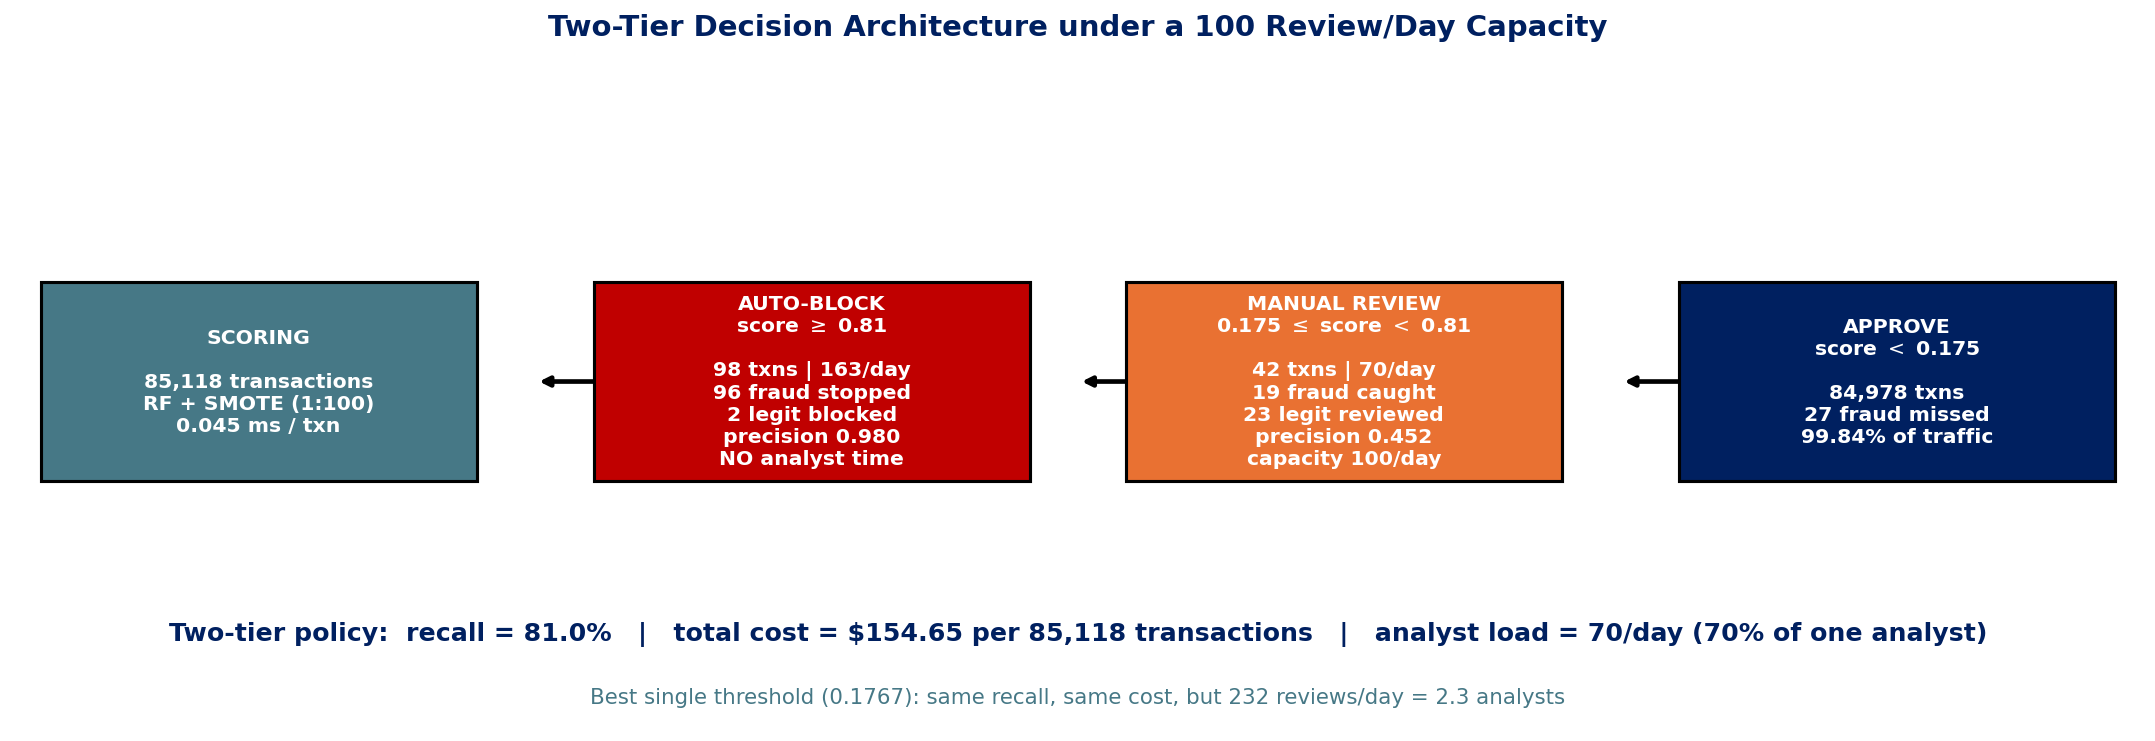
\includegraphics[width=\textwidth]{Images/charts/s9_two_tier_diagram.png}
\caption{Recommended two-tier decision architecture. Auto-blocking above 0.810
consumes no analyst time; only the 0.175--0.810 band counts against the
100-review-per-day capacity, and it amounts to 70 transactions per day.}
\label{fig:twotier}
\end{figure}

\subsection{Scalability and Latency}

\begin{table}[h!]
\centering
\caption{Inference latency and annual compute cost at four transaction
volumes, assuming USD 0.05 per CPU-hour.}
\label{tab:scale}
\begin{tabular}{rrrrr}
\toprule
\textbf{Transactions/day} & \textbf{RF CPU-s/day} & \textbf{RF CPU-h/year} & \textbf{XGB CPU-h/year} & \textbf{RF cost/year} \\
\midrule
100{,}000 & 4.5 & 0.46 & 0.052 & \$0.02 \\
500{,}000 & 22.5 & 2.28 & 0.260 & \$0.11 \\
1{,}000{,}000 & 45.0 & 4.56 & 0.519 & \$0.23 \\
10{,}000{,}000 & 450.1 & 45.63 & 5.192 & \$2.28 \\
\bottomrule
\end{tabular}
\end{table}

The final model scores at \textbf{0.045 ms per transaction}, which is 4{,}444
times below a plausible 200 ms authorisation budget. Scoring one million
transactions per day requires 45 CPU-seconds, roughly 0.8 minutes of
wall-clock time; even ten million per day requires only 7.5 minutes. The
annual compute cost at that scale is under USD 2.30. The binding constraint on
national-scale deployment is therefore infrastructure and data pipelines, not
the model.

Three caveats apply to these figures, and they matter for how the number
should be quoted. First, the latency was measured \emph{in-process} on a single
machine with the model already loaded; it excludes feature engineering,
deserialisation, network transport and any queueing, and it is a
\emph{per-transaction} figure rather than a \emph{throughput} figure under
concurrent load. Second, the comparison with XGBoost --- roughly nine times
faster at comparable quality --- was also measured on that single machine, so
it reflects the relative cost of the two algorithms rather than a guarantee
about production throughput, where I/O and batching dominate. Third, the
latency figure covers model scoring only; SHAP \emph{explanations} are
computed on demand for the 163 auto-blocked and 70 reviewed transactions per
day, not for the full stream, but a bank that wanted explanations for every
decision would face a different bill. We therefore present the latency figure
as evidence that the \emph{algorithm} is not the bottleneck, not as a
capacity plan.

\subsection{What Each Imbalance Technique Costs}

\begin{table}[h!]
\centering
\caption{Average total cost at the 95\% precision constraint, aggregated by
imbalance technique over the configurations that achieve it. Note that the
\emph{mean} and the \emph{best} cost rank the techniques differently.}
\label{tab:techcost}
\begin{tabular}{lrrr}
\toprule
\textbf{Technique} & \textbf{Mean cost} & \textbf{Best cost} & \textbf{Mean recall} \\
\midrule
SMOTE + ENN & \textbf{\$219.50} & \$214.05 & \textbf{0.718} \\
class\_weight = balanced & \$253.92 & \$197.70 & 0.674 \\
SMOTE & \$301.50 & \textbf{\$170.45} & 0.612 \\
No resampling & \$342.63 & \$170.45 & 0.559 \\
\textbf{Random Undersampling} & \$724.85 & \$703.05 & 0.063 \\
\bottomrule
\end{tabular}
\end{table}

Table~\ref{tab:techcost} must be read with care, because the mean and the best
tell different stories and it is easy to conflate them. \emph{By mean cost},
SMOTE-ENN is the most economical technique and SMOTE is only third. \emph{By
best achievable cost}, SMOTE and no resampling tie at USD 170.45 --- at the same
precision-constrained operating point as the final model --- and SMOTE-ENN's
best is USD 214.05.

Random Undersampling is the one unambiguous result: it is the most expensive
technique by a wide margin, averaging USD 724.85, which is 2.4 times the mean
cost of SMOTE and 4.3 times its best achievable cost. Its precision-constrained
recall of 0.063 reflects the loss of the majority-class evidence the model
needs. Random Undersampling is also the only technique that degraded every
model family it was paired with; SMOTE, by contrast, slightly \emph{lowered}
Average Precision for Decision Tree, Logistic Regression and XGBoost while
raising it substantially for Random Forest.

\subsection{Sensitivity to the Review-Cost Assumption}
\label{sec:sensitivity}

Because the USD 0.30 review cost is our own assumption rather than a published
figure, we re-derived the cost-minimising threshold for a range of alternative
review costs. The result is reassuring for the qualitative conclusions but
notable for the operating point: as review becomes more expensive, the
optimal threshold rises sharply, because each additional false alarm costs
more than the fraud it might catch.

\begin{table}[h!]
\centering
\caption{Sensitivity of the cost-minimising operating point to the assumed
cost of one manual review. The threshold rises from 0.0405 to 0.4605 as the
review cost increases twenty-fold. Every row is an \emph{unconstrained} cost
optimum whose review workload (193.3 to 685.0 transactions per day) exceeds
the 100-review-per-day capacity of a single analyst, which is why no single
threshold is deployable at any review price, whereas the two-tier policy of
Section~\ref{sec:twotier} stays feasible at every price because auto-blocking
consumes no analyst time.}
\label{tab:sens}
\scriptsize
\setlength{\tabcolsep}{4pt}
\begin{tabular}{rrrrr}
\toprule
\textbf{Review cost} & \textbf{Optimal threshold} & \textbf{Recall} & \textbf{Precision} & \textbf{Workload/day} \\
\midrule
\$0.10 & 0.0405 & 0.8662 & 0.2993 & 685.0 \\
\$0.30 (assumed) & 0.0905 & 0.8310 & 0.6519 & 301.7 \\
\$0.50 & 0.1705 & 0.8099 & 0.8214 & 233.3 \\
\$1.00 & 0.3135 & 0.7958 & 0.8898 & 211.7 \\
\$2.00 & 0.4605 & 0.7817 & 0.9569 & 193.3 \\
\$5.45 & 0.4605 & 0.7817 & 0.9569 & 193.3 \\
\bottomrule
\end{tabular}
\end{table}

\begin{figure}[h!]
\centering
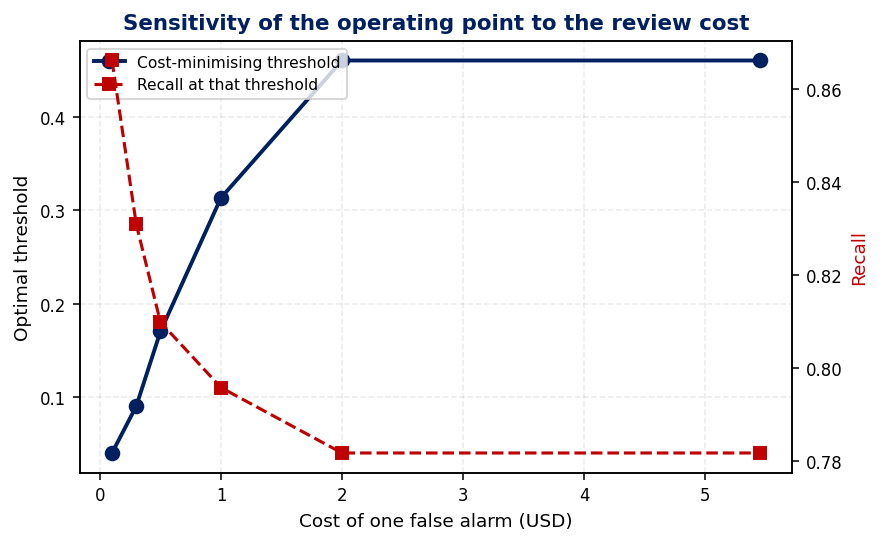
\includegraphics[width=0.55\textwidth]{Images/charts/s10_sensitivity_review_cost.png}
\caption{Sensitivity of the operating point to the review-cost assumption. As
review becomes more expensive the bank should demand higher precision and
should accept lower recall; the ranking of the model against rule-based
systems is unaffected.}
\label{fig:sens}
\end{figure}

Three conclusions survive every row of Table~\ref{tab:sens}. First, the
\emph{ranking} of configurations is stable: Random Undersampling remains the
worst technique and the two-tier architecture remains feasible because
auto-blocking costs no analyst time at any review price. Second, the recall
that can be sustained is remarkably flat between \$0.30 and \$2.00 (0.83 down
to 0.78), so the headline result does not depend delicately on the exact
assumption. Third, the \emph{volume} of review changes by more than a factor
of three, which is precisely why the two-tier design matters: it shifts work
from the analyst onto software, and that benefit is largest exactly where the
review cost is highest.

\subsection{Answers to the Seven Business Questions}

\begin{table}[h!]
\centering
\caption{Responses to the seven business questions posed in the project brief.}
\label{tab:qa}
\small
\begin{tabular}{p{1.1cm}p{6.6cm}p{7.3cm}}
\toprule
\textbf{\#} & \textbf{Question} & \textbf{Answer} \\
\midrule
1 & Which model attains the highest F1 on the test set? & \textbf{Random Forest + SMOTE (1:100)}: F1 = 0.8605 (P 0.9569, R 0.7817) \\
2 & What recall is achievable at a minimum precision of 95\%? & \textbf{78.17\%} at the test-tuned threshold, \textbf{73.24\%} leakage-free (out-of-fold tuning); the recommended two-tier policy reaches \textbf{80.99\%} \\
3 & Which features contribute most? & \texttt{Amount} (SHAP rank 1, permutation rank 2), \texttt{Amount\_log} (1, 2), \texttt{V14} (3, 3); \texttt{Day} reaches SHAP rank 5 \\
4 & At 100 manual reviews per day, what is the operating cost and the saving? & A single threshold needs 1.9 analysts. The \textbf{two-tier policy needs only 0.7 analyst} (70 reviews/day) and reaches \textbf{81.0\% recall at \$154.65} per 85{,}118 transactions --- an \textbf{80\% reduction} in annual fraud cost versus deploying no model (USD 470{,}789 $\rightarrow$ USD 94{,}079 per year) \\
5 & Score all transactions, or only those above an amount threshold? & \textbf{Score all.} Only 3.2\% of the traffic lies above \$500, and it contains just \textbf{9.9\%} of all fraud --- an amount gate discards 90\% of the fraud before scoring; roughly two thirds of the missed frauds are below \$10 \\
6 & What is the compute cost and latency at full scale? & \textbf{0.045 ms/transaction}, 4{,}444$\times$ headroom against a 200 ms budget; 1 M transactions/day = 45 CPU-seconds; compute under \textbf{USD 2.30/year} at 10 M/day \\
7 & How do imbalance techniques affect business cost? & \textbf{Random Undersampling is the most expensive} (mean USD 724.85, 4.3$\times$ the best achievable SMOTE cost; recall 0.063) and the only technique that degraded every model family. \textbf{SMOTE gives the best ranking} (AUC-PR 0.8055 $\rightarrow$ 0.8239); at the operating point it ties with no resampling at USD 170.45 \\
\bottomrule
\end{tabular}
\end{table}
